\documentclass[a4paper]{exam}

\usepackage{graphicx}
\usepackage{siunitx}
\DeclareSIUnit{\revolution}{rev}
\DeclareSIUnit{\rpm}{\revolution\per\minute}
\DeclareSIUnit{\lightyear}{ly}

\begin{document}

\section*{L3 Physics: Questions for 3.1 (Electrodynamics, DC analysis)}
The first four questions below are from Knight, chapter 28. Questions 5 to 8 are from past exams.

You are reminded that the questions are not necessarily ordered in terms of difficulty.

\begin{questions}
  \question
    \begin{parts}
      \part What is the equivalent resistance between points a and b in the following circuit fragment?

            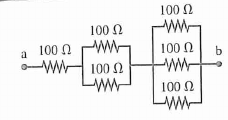
\includegraphics[width=0.3\textwidth]{ex2827}
      \part The \SI{10}{\ohm} resistor in the following circuit fragment is dissipating \SI{40}{\watt}. How much
            power is being dissipated by the two other resistors?

            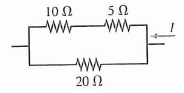
\includegraphics[width=0.3\textwidth]{ex2829}
      \part What are the emf and internal resistance of the battery in the following circuit?

            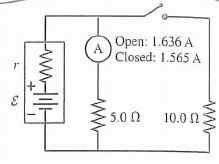
\includegraphics[width=0.3\textwidth]{p2847}

    \end{parts}
  \question
    \begin{parts}
      \part What value resistor will discharge a \SI{2.0}{\micro\farad} capacitor to 20\% of its initial charge in \SI{4}{\milli\second}?
      \part A capacitor is discharged through a \SI{200}{\ohm} resistor. The discharge current decreases to 20\% of its initial value
            in \SI{2.0}{\milli\second}. What is the value of the capacitance?
    \end{parts}
  \question The switch in the following circuit has been closed for a very long time.

            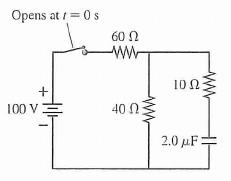
\includegraphics[width=0.3\textwidth]{cp2880}

    \begin{parts}
      \part What is the charge on the capacitor?
      \part The switch is opened at time $ t = \SI{0}{\second} $. At what time has the charge on the capacitor decreased to 10\% of its initial value?
    \end{parts}
  \clearpage
  \question What power is dissipated by the \SI{2}{\ohm} resistor in the following circuit?

            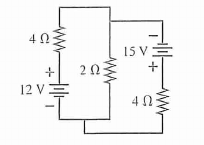
\includegraphics[width=0.3\textwidth]{cp2878}

  \question Casey sets up a battery, a switch, and a \SI{3.00}{\ohm} light bulb in series. The battery voltage is
            measured to be \SI{6.02}{\volt} when the switch is open.  However, when the switch is closed,
            Casey notices that the battery voltage drops to \SI{5.85}{\volt}.
    \begin{parts}
      \part Explain why the battery voltage is less when the switch is closed.
      \part Casey measures the current through the circuit to be \SI{1.89}{\ampere}. State the emf, and show that
            the internal resistance of the battery is approximately \SI{0.09}{\ohm}.
      \part Casey now adds a capacitor in series with the battery and closes the switch. Casey measures the
            voltage across the capacitor as it charges.

            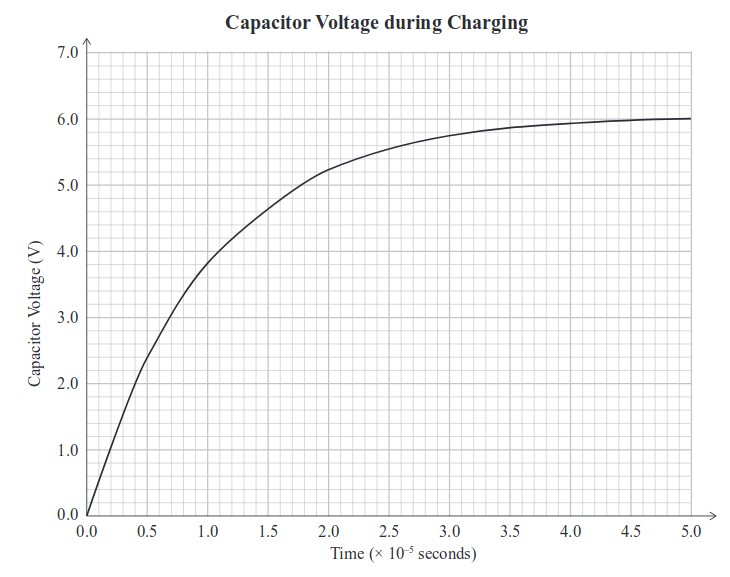
\includegraphics[width=0.6\textwidth]{capacitor-nzqa2018}

            Using information from the graph, determine the capacitance of the capacitor.
      \part Casey discharges the capacitor, removes the light bulb, and begins to charge the capacitor
            again. Casey predicts that, by removing the light bulb, less energy will be converted to light
            and heat, and so the capacitor will charge more quickly, and have more stored energy once fully charged.
            Use physical reasoning to discuss each aspect of Casey’s prediction.

            You should discuss, with explanations:
            \begin{itemize}
              \item whether the capacitor will charge more quickly than before
              \item whether less energy will be converted to light and heat during the charging process without the light bulb
              \item whether more energy will be stored in the fully charged capacitor.
            \end{itemize}
    \end{parts}
  \question Show that the force of gravitational attraction between a pair of electrons is about \num{1e-43} times the force of electrostatic repulsion.

            The force of electrostatic repulsion between two charges $ q_1 $ and $ q_2 $, separated by a distance $ r $, is
            \begin{displaymath}
              F = k\frac{q_1 q_2}{r^2}
            \end{displaymath}
            where $ k $ is Coulomb's constant. (Some useful data may be found at the end of this problemset.)
  \question A resistance of \SI{4.0}{\ohm} is connected across a cell of internal resistance $ r $. The \SI{4.0}{\ohm} resistor
            dissipates energy at \SI{16}{\watt}. The \SI{4.0}{\ohm} resistor is replaced by a \SI{1.0}{\ohm} resistor, which
            also dissipates energy at \SI{16}{\watt}. Show that the source voltage must be \SI{12}{\volt}.
  \question
    \begin{parts}
      \part Describe the electrical properties required for a material to act as a dielectric.
      \part A capacitor containing a dielectric is initially charged and then disconnected from a battery. The capacitor then has its dielectric removed.
        \begin{subparts}
          \subpart Explain why work has to be done to remove the dielectric.
          \subpart Show that the minimum work required to remove the dielectric is
                   \begin{displaymath}
                     \frac{1}{2} C_F V_F^2 \left(\frac{\varepsilon_r - 1}{\varepsilon_r}\right),
                   \end{displaymath}
                   where $ C_F $ is the capacitance of the capacitor with dielectric removed, $ V_F $ is the final potential difference, and
                   $ \varepsilon_r $ is the dielectric constant.
        \end{subparts}
      \part If the capacitor is still connected to the battery when the dielectric is removed, the energy stored in the capacitor will decrease.
            Despite this reduction in energy, work must still be done to withdraw the dielectric. Explain this apparent contradiction.
      \part If the charged capacitor is held just touching the surface of a liquid dielectric, the dielectric
            will be drawn up into the capacitor.
        \begin{subparts}
          \subpart Explain why the capacitor voltage decreases when this phenomenon takes place.
          \subpart Explain why the liquid dielectric is drawn up into the charged capacitor.
        \end{subparts}
    \end{parts}
\end{questions}

\subsection*{Useful data}
\begin{tabular}{rl}
  Mass of an electron & \SI{9.11e-31}{\kilo\gram}\\
  Charge of an electron & \SI{-1.60e-19}{\coulomb}\\
  Gravitational constant & \SI{6.67e-11}{\newton\metre\squared\per\kilo\gram\squared}\\
  Coulomb's constant & \SI{8.98e9}{\newton\metre\squared\per\coulomb\squared}
\end{tabular}

\vspace*{\fill}
This version: \today

\end{document}
